\documentclass[../../main/main.tex]{subfiles}
\graphicspath{{./figures/}}

\makeatletter
\renewcommand{\@chapapp}{Optique -- chapitre}
\makeatother

% \toggletrue{student}
% \HideSolutionstrue
\toggletrue{corrige}
\renewcommand{\mycol}{black}
% \renewcommand{\mycol}{gray}

\begin{document}

\chapter{Propagation de la lumi\`ere}

\vfill

\begin{prgm}
	\begin{tcb}*[sidebyside](ror)"know"{Savoirs}
		\begin{itemize}[label=$\diamond$, leftmargin=10pt]
			\item Définir une onde sinusoïdale/monochromatique.
			\item Caractériser une source lumineuse par son spectre.
			\item Relier la longueur d'onde dans le vide et la couleur.
		\end{itemize}
		\tcblower
		\begin{itemize}[label=$\diamond$, leftmargin=10pt]
			\item Connaître la valeur numérique de la célérité de la lumière dans le
			      vide.
			\item Définir l'indice d'un milieu transparent.
		\end{itemize}
	\end{tcb}

	\begin{tcb}*(ror)"how"{Savoir-faire}
		\begin{itemize}[label=$\diamond$, leftmargin=10pt]
			\item Déterminer la longueur d'onde d'un rayonnement dans un milieu à partir
			      de sa longueur d'onde dans le vide.
		\end{itemize}
	\end{tcb}
\end{prgm}

\vfill
\minitoc
\vfill

\newpage

\section{L'onde lumineuse}

\subsection{Nature ondulatoire de la lumière}

\noindent
\begin{minipage}[t]{.48\linewidth}
	La nature de la lumière a été l'objet de discussions et controverses durant
	des siècles, opposant principalement au \textsc{xvii}\ieme\ \textsc{Newton}
	avec sa théorie corpusculaire et \textsc{Hooke} puis \textsc{Huygens} avec la
	théorie ondulatoire. Le débat s'est clos avec les expériences d'interférences
	de \textsc{Young} et \textsc{Fresnel} (début \textsc{xix}\ieme) notamment,
	prouvant son comportement ondulatoire (nous aurons l'occasion de les réaliser
	nous-mêmes).
	\smallbreak
	Ce n'est cependant qu'à la fin du \textsc{xix}\ieme\ avec les théories
	de \textsc{Maxwell} que cette onde est décrite par la propagation de grandeurs
	électromagnétiques (champ électrique, champ magnétique, et donc pas dans un
	milieu matériel).
\end{minipage}
\hfill
\begin{minipage}[t]{.48\linewidth}
	~
	\vspace*{-20pt}
	\begin{center}
		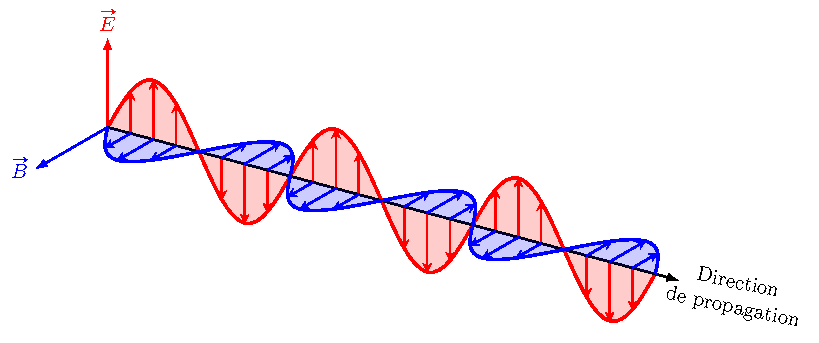
\includegraphics[width=\linewidth]{propagation}
		\captionof{figure}{Représentation des oscillations du champ
			électromagnétique lors de la propagation de la lumière}
		\label{fig:proplum}
	\end{center}
\end{minipage}
\bigbreak
Le \textsc{xx}\ieme\ vint bousculer cette vision en attestant de la dualité
onde-corpuscule des particules élémentaires de l'Univers avec l'avènement de la
physique quantique. Selon les conditions d'études, l'une ou l'autre des visions
sera appliquée.

\subsection{Célérité de la lumière}

\subsubsection{Dans le vide}

En tant qu'onde électromagnétique, la lumière n'est pas une onde mécanique
nécessitant un milieu matériel pour se propager\footnote{À la différence d'une
	vague sur l'eau ou d'une corde de guitare qui se propagent sur un milieu
	matériel.}.
\begin{tcb}(defi){Définition}
	Nous appelons \textit{célérité} de la lumière \textbf{dans le vide}, et
	la notons $c$, la vitesse de l'onde lumineuse.
\end{tcb}
\begin{tcb}[sidebyside](odgr){Valeur}
	La valeur de $c$ est fixée par définition\footnote{Elle n'est donc
		théoriquement plus mesurable, puisque les mesures de distances se basent sur
		la valeur de la célérité de la lumière}, telle que
	\[c = \SI{2.99792458e8}{m.s^{-1}}\]
	\tcblower
	Nous utiliserons et retiendrons cependant la valeur
	\[
		\bsw{
			\boxed{c = \SI{3.00e8}{m.s^{-1}}}
		}
	\]
\end{tcb}

\subsubsection{Dans un milieu}

Elle peut cependant se propager dans certains milieux matériels transparents,
comme l'air, l'eau, le verre… Dans le cadre de la physique de cette année, nous
étudierons des milieux particuliers~:

\begin{tcb}(defi){Définition~: milieu transparent linéaire homogène isotrope (TLHI)}
	\begin{itemize}[leftmargin=66pt]
		\item[\textbf{Transparent}] : \bsw{
			      qui laisse passer la lumière~;
		      }
		\item[\textbf{Linéaire}] : \bsw{
			      dont les sorties sont proportionnelles aux
			      entrées~;
		      }
		\item[\textbf{Homogène}] : \bsw{
			      dont les propriétés physiques sont
			      constantes en tout point du milieu~;
		      }
		\item[\textbf{Isotrope}] : \bsw{
			      dont les propriétés physiques ne
			      dépendent pas de la direction de la lumière dans le milieu.
		      }
	\end{itemize}
\end{tcb}

Lorsque la lumière passe dans un tel milieu, sa vitesse \textbf{diminue}. Nous
caractérisons cette diminution \textit{via} la définition de l'indice optique~:

\begin{tcb}[sidebyside](defi){Définition~: indice optique}
	Nous appelons \textit{indice optique} la grandeur associée à un milieu
	transparent et caractérisant la \textbf{vitesse de la lumière en son sein},
	telle que~:
	\[
		\bsw{
			\boxed{n = \frac{c}{v}}
		}
	\]
	\tcblower
	\tcbsubtitle{\fatbox{Unités}}

	\bsw{
		En tant que rapport de deux grandeurs de même unité, l'indice optique
		n'a pas d'unité.
	}
\end{tcb}

\begin{tcb}[lfnt](rema){Remarque}
	Étant donné que la vitesse de la lumière \textbf{dans le vide} est
	absolue et indépassable, la vitesse de la lumière dans un milieu
	transparent ne peut qu'être plus petite, et donc
	\begin{center}
		\bsw{
			\fbox{
				\textbf{l'indice optique est toujours > 1}
			}
		}
	\end{center}
\end{tcb}

\begin{tcbraster}[raster columns=2, raster equal height=rows]

	\begin{tcb}(impl){Implication}
		Par la définition de l'indice optique, nous déduisons l'expression de la
		vitesse de la lumière dans un milieu par~:
		\[
			\bsw{
				\boxed{v = \frac{c}{n}}
			}
		\]
	\end{tcb}
	\begin{tcb}(odgr)'r'{Ordre de grandeur}
		\begin{tabular*}{\linewidth}{@{\extracolsep{\fill}}lS[table-format=1.2]S[table-format=1.2e1]@{}}
			\toprule
			Milieu  & $n$  & $v [\si{m.s^{-1}}]$ \\
			\midrule
			Vide    & \bsw{\num{1}}    & \bsw{\num{3.00e8}} \\
			Air     & \bsw{\num{1.00}} & \bsw{\num{3.00e8}} \\
			Eau     & \bsw{\num{1.33}} & \bsw{\num{2.30e8}} \\
			Verre   & \bsw{\num{1.5}}  & \bsw{\num{2.00e8}} \\
			Diamant & \bsw{\num{2.4}}  & \bsw{\num{1.25e8}} \\
			\bottomrule
		\end{tabular*}
	\end{tcb}

\end{tcbraster}

\subsubsection{Selon la fréquence}

L'indice optique dépend de la fréquence d'une onde lumineuse, et ainsi la
vitesse de la lumière dans un milieu TLHI aussi. Comme la couleur de la lumière
correspond à la fréquence de l'onde la représentant, cela cause la
\textbf{dispersion} de la lumière\footnote{Pensez par exemple au prisme de Pink
	Floyd.}. Cet effet est cependant souvent négligé car faible par rapport à
d'autres phénomènes.

\subsection{Longueur d'onde d'une onde sinusoïdale}

\begin{tcb}(defi){Définition~: onde sinusoïdale}
	\bsw{
		Une onde sinusoïdale est une onde \textbf{monochromatique}, ce qui
		signifie «~une seule couleur~». Elle est donc décrite par une unique
		valeur de longueur d'onde ou de fréquence, et non pas comme une
		superposition.
	}
\end{tcb}

\begin{tcb}(exem){Exemples}
	Une lumière rouge est monochromatique, et est décrite par une onde lumineuse
	de longueur d'onde $\approx \SI{700}{nm}$. Une lumière \textbf{blanche} ne
	l'\textbf{est pas}, c'est une \textit{superposition} d'ondes sinusoïdales sur
	le domaine du visible.
\end{tcb}

\begin{tcb}(prop){Propriété}
	Une onde lumineuse se caractérise par sa fréquence, appelée $f$ ou
	$\nu$\footnote{Se lit «~nu~».}. En effet, \textbf{la fréquence d'une
		onde est indépendante du milieu traversé}. En revanche, sa
	\textbf{longueur d'onde en dépend}.
\end{tcb}

\begin{tcb}[sidebyside](impl){Implication}
	Avec l'analyse dimensionnelle, on trouve directement qu'une longueur
	d'onde $\lambda$ doit s'écrire
	\bsw{
		\[
			\lambda = \frac{v_{\rm onde}}{f_{\rm onde}}
		\]
	}
	\tcblower
	Or, dans le vide $v_{\rm onde} = c$, et dans un milieu TLHI d'indice
	optique $n$, $v_{\rm onde} = \frac{c}{n}$~; ainsi avec $\lambda_0$ dans
	le vide~:
	\bsw{
		\[
			\boxed{\lambda_0 = \frac{c}{f}}
			\quad\text{et}\quad
			\boxed{\lambda = \frac{c}{n\times f} = \frac{\lambda_0}{n}}
		\]
	}
\end{tcb}

\begin{tcb}(ror){À retenir}
	Ainsi, quand on parle de la longueur d'onde d'une couleur, on parle en réalité
	de sa longueur d'onde \textit{dans le vide}.
\end{tcb}

\begin{figure}[h]
	\centering
	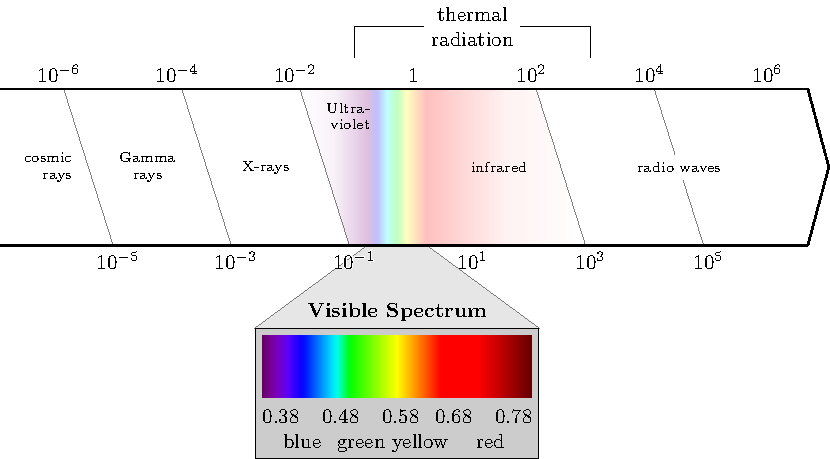
\includegraphics[width=.9\linewidth]{full_spectre}
	\caption{Longueurs d'ondes des ondes monochromatiques \textbf{dans le vide}.}
	\label{fig:lambda_vis}
\end{figure}

\begin{tcb}(exem){Exercice}
	Un laser rouge émet un rayonnement de longueur d'onde dans le vide
	$\lambda_0 = \SI{633}{nm}$. Déterminer sa longueur d'onde $\lambda$ dans du
	verre, d'indice optique $n = \num{1.5}$. Sa couleur change-t-elle~?
	\tcblower
	\bsw{
		D'après ce qui précède, on a
		\begin{gather*}
			\boxed{\lambda = \frac{\lambda_0}{n}}
			\qav
			\left\{
			\begin{array}{rcl}
				\lambda_0 & = & \SI{633}{nm}
				\\
				n         & = & \num{1.5}
			\end{array}
			\right.\\
			\mathrm{A.N.~:}\enskip
			\xul{
				\lambda = \SI{422}{nm}
			}
		\end{gather*}
		Cependant, \textbf{sa couleur ne change pas} puis qu'\xul{une onde est
			caracétrisée par sa fréquence}, qui ne change pas.
	}
\end{tcb}

\section{Sources lumineuses primaires}

On parle de source primaire quand l'objet en question émet directement de la
lumière. Les sources secondaires ne font qu'en renvoyer, par exemple la Lune, la
peau, les arbres…

\subsection{Spectre d'émission}

Pour caractériser un rayonnement électromagnétique, on trace son spectre
d'émission, c'est-à-dire la courbe de l'intensité lumineuse en fonction de la
fréquence (ou longueur d'onde dans le vide).

Les sources primaires sont classées selon leur contenu spectral
qui découle du type de processus d'émission lumineuse~:
\begin{itemize}[leftmargin=120pt]
	\item[\textbf{Sources thermiques}] : \bsw{
		      agitation thermique des atomes~;
	      }
	\item[\textbf{Sources spectrales}] : \bsw{
		      excitation électrique des atomes~;
	      }
	\item[\textbf{Sources LASER}] : \bsw{
		      optimisation de l'émission stimulée de photons.
	      }
\end{itemize}

\subsection{Les sources thermiques}

L'agitation thermique des atomes émet un rayonnement électromagnétique dépendant
de sa température~: c'est le type de rayonnement du Soleil ou des ampoules à
incandescence (chauffage d'un métal qui brille).

\begin{tcb}(defi){Caractéristiques du rayonnement d'un corps chaud}
	\bsw{
		Le spectre d'émission d'une source thermique est une courbe
		\textbf{continue}, étalée autour d'une longueur d'onde d'émission maximale
		$\lambda_{\max}$. Plus la température augmente, plus le spectre se déplace
		vers une fréquence élevée (ou longueur d'onde faible)~: une étoile bleue est
		bien plus chaude qu'une étoile rouge.
	}

\end{tcb}

\begin{tcb}[sidebyside, lefthand ratio=.5](exem){Exemples}
	\begin{itemize}
		\item À température ambiante ($T \approx \SI{300}{K}$), un corps émet
		      dans l'infrarouge (c'est le principe d'une caméra infrarouge)~;
		\item Pour une lampe, le filament est à $T \approx \SI{2800}{K}$. Son
		      maximum est dans l'infrarouge mais son spectre s'étale sur le
		      domaine visible~;
		\item La température de surface du Soleil est de $T \approx
			      \SI{5700}{K}$. Son maximum d'émission est dans le domaine visible.
	\end{itemize}
	\begin{center}
		\pgfspectra[element={H,Fe,Mg,Na},
		absorption, line intensity=40, Imin=.05,
		axis, axis color=white, axis font color=black,
		axis ticks=4, axis unit precision=2,
		axis label text={Longueur d'onde [$\si{nm}$]},
		back=visible10,
		]
		\captionof{figure}{Spectre lumineux que l'on reçoit du Soleil.}
		\label{fig:spec_sun}
	\end{center}
	\tcblower
	\begin{center}
		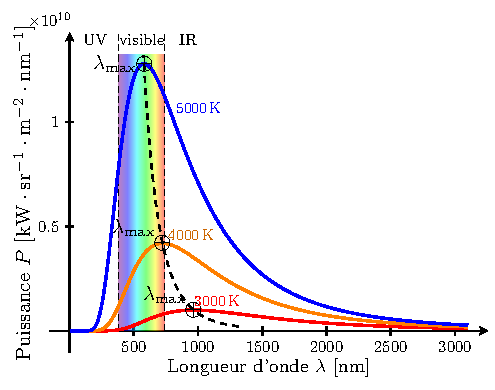
\includegraphics[width=\linewidth]{blackbody}
		\captionof{figure}{Spectre d'émission d'un corps chaud selon quelques
			températures.}
		\label{fig:cps_chaud}
	\end{center}
\end{tcb}

\subsection{Les sources spectrales}

Une lampe spectrale contient un élément chimique sous forme de gaz, et deux
électrodes de part et d'autre du contenant génère des décharges électriques qui
excitent les atomes. C'est un état instable. En revenant dans leur état
fondamental, ils émettent des photons à une énergie précise correspondant à la
différence des niveaux d'énergie quantiques de l'élément ($f = \frac{\Delta
		E}{h}$~; voir chapitre introduction à la physique quantique).

\begin{tcb}(defi){Caractéristiques du rayonnement spectral}
	\bsw{
		Le spectre d'émission d'un rayonnement spectral est composé de
		\textbf{pics d'intensités} faiblement élargis. Les longueurs d'onde de ces
		pics sont \textbf{caractéristiques de l'élément} excité~; c'est de cette
		manière qu'on peut déterminer la composition atmosphérique des exoplanètes
		ou caractériser les étoiles.
	}
\end{tcb}
\begin{tcb}[sidebyside, righthand width=.5\linewidth](exem){Exemples}
	On trouve des lampes au néon, de couleur rouge~; des lampes au mercure, de
	couleur bleue~; des lampes à sodium, dans l'orange… On utilisera
	principalement ces deux dernières en laboratoire.
	\tcblower
	\begin{center}
		\pgfspectra[element=Hg,
		axis, axis color=white, axis font color=black,
		axis ticks=4, axis unit precision=2,
		axis label text={Longueur d'onde [$\si{nm}$]},
		back=white,
		label, label position=north west,
		label before text=Spectre d'émission de~,
		label after text=\ :]
		\captionof{figure}{Spectre d'émission d'une lampe à vapeur de mercure.}
		\label{fig:lamp_spec}
	\end{center}
\end{tcb}

\subsection{Le LASER}
LASER est l'acronyme de \textit{Light Amplification by Stimulated Emission of
	Radiations}, c'est-à-dire «~amplification de la lumière par émission stimulée de
radiations~». Il est composé d'une cavité remplie d'un milieu recevant de
l'énergie, excité par une source extérieur, et fermée par deux miroirs. Celui de
la face de sortie est légèrement transparent.

La lumière passe au travers du milieu qui réémet de la lumière sans atténuer la
première, et grâce au miroir le tout est réfléchi pour permettre de nombreux
aller-retours, amplifiant l'intensité lumineuse à chaque passage.

\begin{tcb}(defi){Caractéristiques du rayonnement LASER}
	\bsw{
		Le spectre du laser ne contient qu'\textbf{une seule raie extrêmement
			fine}, bien plus fine que celle des sources spectrales. C'est l'exemple le
		plus proche d'une réelle source monochromatique.
	}
\end{tcb}

\begin{tcb}[sidebyside, righthand width=.5\linewidth](exem){Exemple}
	Un laser hélium-néon donne un faisceau rouge de longueur d'onde dans le vide
	$\lambda_0 = \SI{632.8}{nm}$.
	\tcblower
	\begin{center}
		\pgfspectra[lines={632.8},
		axis, axis color=white, axis font color=black,
		axis ticks=4, axis unit precision=2,
		axis label text={Longueur d'onde [$\si{nm}$]},
		back=white,
		label, label position=north west,
		label before text=Spectre d'émission d'un laser \ce{He-Ne}]
		\captionof{figure}{Spectre d'émission d'un laser hélium-néon.}
		\label{fig:laser_spec}
	\end{center}
\end{tcb}
\begin{tcb}(impo){Attention}
	Si la puissance totale du faisceau est communément assez faible ($P \approx
		\SI{1}{mW}$), sa surface l'est également ($S \approx \SI{1}{mm^2}$). La
	puissance \textit{surfacique} est donc en réalité très grande, et
	particulièrement dangereuse pour l'œil. On veillera donc à ne jamais le
	diriger vers un œil, mais aussi à éviter toute réflexion involontaire
	(notamment sur tout métal~: bijou, tige de support…).
\end{tcb}

\end{document}
